\chapter{Implementierung}



\section{App zur LED-Steuerung} \label{impl_steuer_app}

\subsection{Aufbau der Anwendung}
Die Anwendung soll auf der Startseite die Ansicht eines Colorpickers darstellen, sodass sofort nach Start der App eine Farbe ausgewählt werden kann. Diese Farbe wird sofort ohne Bestätigung an die ausgewählte LED Leiste gesendet. \\
Über einen Navigation-Drawer vom linken Bildschrim sind neben dem bereits ausgewählten Reiter \textit{Colorpicker} noch die Reiter \textit{Effects}, \textit{State} und \textit{Settings} auswählbar. Diese haben folgende Funktionalitäten:
\begin{description}
	\item[Effects] Zeigt alle möglichen Effekte, die der Home Manager momentan umsetzen kann. Durch einen Klick auf die entsprechende Schaltfläche wird der Effekt auf der ausgewählten LED Leiste wiedergegeben.
	\item[State] Diese Ansicht zeigt die Zustände (Farbe, Effekt) der LEDs, die sich momentan im Netzwerk befinden. Diese Liste wird vom Home Manager geliefert.
	\item[Settings] Hier werden die nötigen Einstellungen getroffen. Momentan zählen hierzu die Adresse und der Port, unter der der Message-Broker erreichbar ist. Zusätzlich werden hier die Topics der einzelnen LEDs festgelegt, damit diese in anderen Teilen einfach ausgewählt werden können.
\end{description}

\subsection{Funktionale Anforderungen}

Die Funktionen wurden teilweise schon im vorherigen Abschnitt erläutert. Im Allgemeinen kann die App als eine grafische Oberfläche zur Erstellung \& dem Versenden der verschiedenen JSON-Nachrichten gesehen werden. Die App stellt einen grafischen Colorpicker dar, wovon sich der Benutzer eine Farbe aussuchen kann. Sobald diese ausgewählt wurde, wird ein Listener aufgerufen, der den Farbcode des Colorpickers in RGB umwandelt und diese Informationen über entsprechende Objekte in ein JSON-Objekt umwandelt. Dieses wird mit dem vorher ausgewählten Topic, das über einen Button repräsentiert wird, auf das Netzwerk geschrieben, wodurch der Rest der Infrastruktur die LED zum Leuchten bringt. \\
Die JSON-Dokumente werden dabei von einer selbst erstellten Klasse \textit{JsonBuilder} erstellt. Diese ist nach dem Builder-Pattern aufgebaut, sodass möglich einfach ein neues JSON-Dokument erstellt und in neue Komponenten eingepflegt werden kann.\\
Beim Reiter \textit{Effects} werden entsprechend andere Teile des JSON-Dokuments eingefügt, sodass der Mikrocontroller diese versteht und die Effekte wie Regenbogen darstellt. \\
Im Reiter \textit{State} befindet sich eine Liste aller in der App hinterlegten LEDs. Hier wird immer ein Paar aus dem Namen der LED, welcher in den anderen Komponenten angezeigt wird, und dem Topic der LED hinterlegt. Das Hinzufügen wird über einen Floating Action Button vorgenommen, der einen Dialog öffnet, in dem die Informationen eingetragen werden. Einzelne LEDs können mit einem langen Klicken des Elements einfach gelöscht werden. \\
Die letzte Seite \textit{Settings} beinhaltet die Verbindungsparameter, des Message Brokers im Netzwerk. Hier wird die IP und der Port des Servers eingetragen, welche in den Shared Preferences abgelegt und im Rest der Anwendung verwendet werden.


\section{Implementierung der Timer-App} \label{impl_timer_app}
Neben der Steuerungs-App für die LED-Leisten wurde eine weitere Android Applikation entwickelt, welche abhängig vom Fortschritt eines Timers eine LED-Leiste als Fortschrittsanzeige ansteuert.\\
Für eine Verwendung auf einem Tablet in einer Küche ist es wichtig, mehrere parallele Timer zu erstellen und diese auf einer Seite gleichzeitig laufen zu lassen. Bei der Entwicklung sollte berücksichtigt werden, dass auch Benutzer ohne Smart Home Infrastrukutur die App verwenden können. Hierfür wird zwischen den beiden Flavors \gf{default} und \gf{mqtt} unterschieden. Die MQTT Flavor enthält alle Funktionalitäten der normalen Applikation und zusätzlich Funktionalitäten zur Integration in das Smart Home System.

\subsection{Funktionale Anforderungen}
Die Applikation soll folgende Anforderungen zuverlässig erfüllen:
\begin{itemize}
	\item Mehrere Timer erstellen und zeitgleich ablaufen zu lassen. Dabei sollen mehrere Timer gleichzeitig sichtbar sein.
	\item Beim Ablauf eines Timers soll visuell und akustisch auf den Ablauf hingewiesen werden.
	\item Auch beim Schließen der Applikation sollen die Timer im Hintergrund weiterlaufen.
\end{itemize}
Zusätzlich sollen bei Verbindung mit einem MQTT-Broker folgende Funktionalitäten umgesetzt werden (nur in der Flavor \gf{mqtt}):
\begin{itemize}
	\item Konfigurieren eines MQTT Servers und eine automatische Verbindung mit dem Server bei App-Start
	\item Die Auswahl eines Timers in der App überträgt automatisch den aktuellen Fortschritt (Prozentual die abgelaufene Zeit zu der restlichen Zeit) an eine LED Kette. Hierbei wird die LED-Leiste in zwei Teile unterteilt, welche in verschiedenen Farben angezeigt werden
	\item Beim Ablauf eines Timers signalisiert die LED Leiste, dass ein Timer abgelaufen ist. Dies wird durch eine blinkende LED-Leiste repräsentiert.
\end{itemize}

\subsection{Aufbau der Anwendung}
Wie in Diagramm \ref{fig:timerapparchitektur} gezeigt, besteht die App aus zwei Teilen. Der auch im Hintergrund laufende Service beinhaltet die Logik des sekündlichen Herunterzählens und verwaltet alle Timer. Die Benutzeroberfläche zeigt diese Werte in einem GridView an, wobei der Benutzer auch über die UI die Timer ändern kann. Das eigentliche Ändern der Objekte wird allerdings wieder von dem Service gemacht.
\begin{figure}
	\centering
	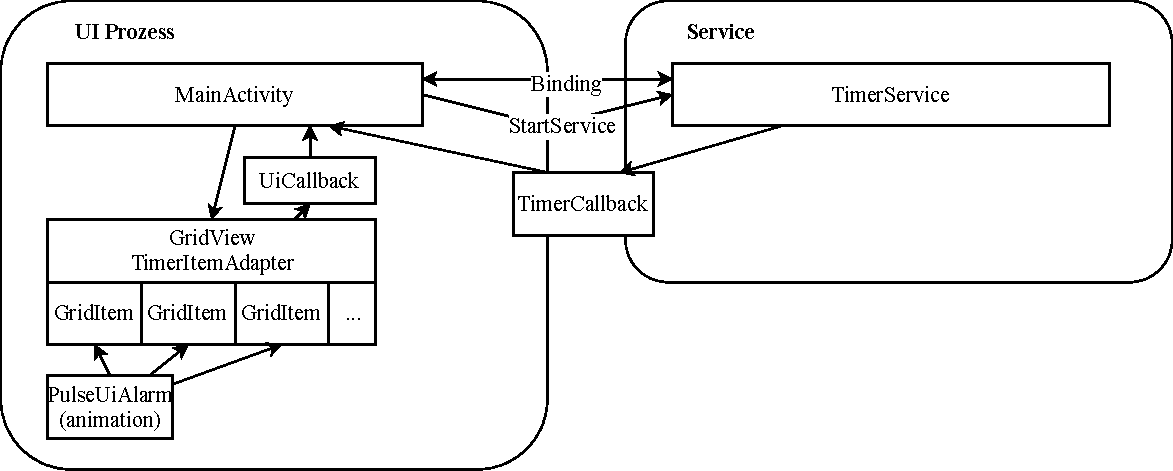
\includegraphics[width=\linewidth]{../images/timer_app_architektur}
	\caption[Timer App Überblick]{Timer App Überblicksarchitektur}
	\label{fig:timerapparchitektur}
\end{figure}


\section{Mikrocontroller} \label{impl_mikrocontroller}
Das in C geschriebene Programm für die einzelnen LED Steuereinheiten wurde als \gf{thin client} umgesetzt. Das heißt, dass nur möglichst einfache Funktionen auf dem Mikrocontroller ausgeführt werden und die komplette Logik auf die steuernden Clienten (siehe \ref{impl_steuer_app} und \ref{impl_timer_app}) und dem Manager (siehe \ref{home_manager}) verschoben werden.\\
Mit der Arduino PubSubClient MQTT Library hört der Mikrocontroller ständig, ob eine neue Nachricht auf ein relevantes Topic angekommen ist. Wenn eine Nachricht ankommt, wird diese durch die \gf{ArduinoJson} Library geparsed und die Werte ausgelesen. Anschließend werden die verarbeiteten Werte mittels der Adafruit Neopixel Library auf die digitalen LEDs geschrieben. Sobald alle LEDs neu beschrieben wurden, hört der Mikrocontroller wieder auf neue Nachrichten vom MQTT Broker.

%\section{Home Manager Modul} \label{home_manager}
%Das Home Manager Modul ist eine Serverkomponente, die Funktionen ausübt, die nicht vom Clienten direkt ausgeführt werden können oder einen erheblichen Mehraufwand der Clientapplikationen bedeuten würde. Der Manager hat mehrere Funktionen, die sich in folgende drei Klassen einteilen lassen.
%\begin{description}
%	\item [Ereignisabhängige Funktionen] können vom Manager verwaltet und ausgeführt werden. Das einfachste Beispiel sind LEDs, die zu einer bestimmten Zeit angeschaltet werden sollen. Hierbei soll ein Clientgerät nur den Auftrag geben, die LEDs anzumachen aber keine Nachricht direkt an die LEDs senden. Hierdurch ist es möglich ein Handy Nachts im Flugzeugmodus zu haben und trotzdem zu einer bestimmten Uhrzeit von langsam angehenden LEDs geweckt zu werden.\\
%	Andere Ereignisse könnten von internen Triggern ausgeführt werden oder von Diensten wie If-This-Then-That gesteuert werden. Diese Funktionalität soll ich Umfang der Projektarbeit sein.
%	\item [Statusüberblick Funktionen] verhelfen allen Geräten synchron mit dem aktuellen Zustand der LEDs zu bleiben. Der Manager notiert bei jeder Änderung von einem Ausgabegerät den neuen Zustand und speichert diesen in einer Datenbank. Wenn sich ein neues Gerät anmeldet, kann dieses die Informationen zu anderen Geräten vom Manager erfragen.
%\end{description}